\documentclass[a4paper]{article}
\usepackage{geometry}
%\usepackage[nostamp,tikz,svg]{moodle}
\usepackage[handout,nostamp,tikz,svg]{moodle}
\pagestyle{empty}
 \geometry{
 a4paper,
 total={175mm,260mm},
 left=15mm,
 top=15mm,
 }

\usepackage{fontspec}
\usepackage{graphicx}
\usepackage{hyperref,babel}
\usepackage[cm]{fullpage}
\usepackage{fancyvrb}

\pagestyle{empty}

\begin{document}
\begin{quiz}{Capitolo 2}

\begin{multi}[points=1,shuffle,multiple,]{2.1-1 Il paradigma client-server.}
\textbf{2.1-1 Il paradigma client-server.} Quali delle seguenti caratteristiche sono associate a un approccio client-server per la strutturazione delle applicazioni di rete (in opposizione a un approccio P2P)?
\item[fraction=33.33333] C'è un server che è sempre acceso.
\item Non c'è un server che è sempre acceso.
\item[fraction=33.33333] C'è un server con un noto indirizzo IP.
\item Un processo richiede un servizio da chi contatta e fornirà un servizio ai processi che lo contattano.
\item[fraction=33.33333] HTTP utilizza questa struttura.
\end{multi}

\begin{multi}[points=1,shuffle,multiple]{2.1-2 Il paradigma peer-to-peer (P2P).}
\textbf{2.1-2 Il paradigma peer-to-peer (P2P).} Quali delle seguenti caratteristiche sono associate a un approccio P2P per la strutturazione delle applicazioni di rete (in opposizione a un approccio client-server)?
\item C'è un server che è sempre acceso.
\item[fraction=50] Non c'è un server che è sempre acceso.
\item C'è un server con un noto indirizzo IP.
\item[fraction=50] Un processo richiede un servizio da chi contatta e fornirà un servizio ai processi che lo contattano.
\item HTTP utilizza questa struttura.
\end{multi}

\begin{multi}[points=1,shuffle,multiple]{2.1-3 Servizio UDP.}
\textbf{2.1-3 Servizio UDP.} Quando un'applicazione utilizza una socket UDP, quali servizi di trasporto vengono forniti all'applicazione da UDP? Selezionare tutte le opzioni valide.
\item \emph{Garanzia di throughput}. La socket può essere configurata per fornire una garanzia di throughput minimo tra mittente e ricevente.
\item \emph{Trasferimento dati privo di perdite}. Il servizio trasferirà in modo affidabile tutti i dati al ricevente, recuperando i pacchetti persi nella rete a causa di overflow nei buffer dei router.
\item \emph{Controllo del flusso}. Il servizio fornito garantirà che il mittente non invii troppo rapidamente da saturare i buffer del ricevente.
\item \emph{Consegna in tempo reale}. Il servizio garantirà che i dati saranno consegnati al ricevente entro un limite di tempo specificato.
\item* \emph{Servizio a ``best-effort''}. Il servizio farà il massimo sforzo per consegnare i dati alla destinazione, ma non garantisce che un particolare segmento di dati arriverà effettivamente.
\item \emph{Controllo della congestione}. Il servizio controllerà i mittenti in modo che non inviino collettivamente più dati di quanto possano gestire i collegamenti nella rete.
\end{multi}

\begin{multi}[points=1,shuffle,multiple]{2.1-4 Servizio TCP.}
\textbf{2.1-4 Servizio TCP.} Quando un'applicazione utilizza una socket TCP, quali servizi di trasporto vengono forniti all'applicazione da TCP? Selezionare tutte le opzioni valide.
\item \emph{Garanzia di throughput}. La socket può essere configurata per fornire una garanzia di throughput minimo tra mittente e ricevente.
\item[fraction=33.33333] \emph{Trasferimento dati privo di perdite}. Il servizio trasferirà in modo affidabile tutti i dati al ricevente, recuperando i pacchetti persi nella rete a causa di overflow nei buffer dei router.
\item[fraction=33.33333] \emph{Controllo del flusso}. Il servizio fornito garantirà che il mittente non invii troppo rapidamente da saturare i buffer del ricevente.
\item \emph{Consegna in tempo reale}. Il servizio garantirà che i dati saranno consegnati al ricevente entro un limite di tempo specificato.
\item \emph{Servizio a ``best-effort''}. Il servizio farà il massimo sforzo per consegnare i dati alla destinazione, ma non garantisce che un particolare segmento di dati arriverà effettivamente.
\item[fraction=33.33333] \emph{Controllo della congestione}. Il servizio controllerà i mittenti in modo che non inviino collettivamente più dati di quanto possano gestire i collegamenti nella rete.
\end{multi}

\begin{multi}[points=1,shuffle,multiple]{2.2-01 ``HTTP è stateless.''}
\textbf{2.2-01 ``HTTP è stateless.''} Cosa intendiamo quando diciamo ``HTTP è stateless''? Nella risposta a questa domanda, assumere che i cookie non siano utilizzati. Selezionare tutte le risposte valide.
\item Il protocollo HTTP non è gestito da uno stato.
\item Un \emph{client} HTTP non ricorda nulla di quanto è accaduto durante le fasi precedenti nell'interazione con un server HTTP.
\item* Un server HTTP non ricorda nulla di quanto è accaduto durante le fasi precedenti nell'interazione con un \emph{client} HTTP.
\item Un \emph{client} HTTP non ricorda le identità dei server con cui ha interagito.
\item Diciamo questo quando un server HTTP non è operativo.
\end{multi}

\begin{multi}[points=1,shuffle]{2.2-02 Cookie HTTP.}
\textbf{2.2-02 Cookie HTTP.} A cosa serve un cookie HTTP?
\item* Un cookie è un codice utilizzato da un server, trasportato su una richiesta HTTP del client, per accedere alle informazioni che il server aveva precedentemente memorizzato su un'interazione precedente con questo \emph{browser} Web. Nota: Pensare alla distinzione tra un \emph{browser} e una \emph{persona}.
\item Un cookie è utilizzato per falsificare l'identità del client verso un server HTTP.
\item Un cookie è un codice utilizzato da un server, trasportato su una richiesta HTTP del client, per accedere alle informazioni che il server aveva precedentemente memorizzato su un'interazione precedente con questa \emph{persona}. Nota: Pensare alla distinzione tra un \emph{browser} e una \emph{persona}.
\item Un cookie è un codice utilizzato da un client per autenticare l'identità di una persona verso un server HTTP.
\item I cookie vengono utilizzati alla fine di una transazione, per indicare la fine della transazione.
\end{multi}
            
\begin{multi}[points=1,shuffle]{2.2-03 Il messaggio HTTP GET.}
\textbf{2.2-03 Il messaggio HTTP GET.} Qual è lo scopo del messaggio HTTP GET?
\item* Il messaggio di richiesta HTTP GET viene utilizzato da un client web per chiedere a un server web d'inviare l'oggetto richiesto.
\item Il messaggio di richiesta HTTP GET viene utilizzato da un client web per inviare un oggetto a un server web.
\item Il messaggio di richiesta HTTP GET viene inviato da un server web a un client web per ottenere l'identità del client web.
\item Il messaggio di richiesta HTTP GET viene inviato da un server web a un client web per ottenere la successiva richiesta dal client web.
\end{multi}


\begin{multi}[points=1,shuffle]{2.2-04 HTTP GET condizionale.}
\textbf{2.2-04 Richiesta HTTP GET condizionale.} Qual è lo scopo del messaggio di richiesta HTTP GET condizionale?
\item* Per consentire a un server d'inviare l'oggetto richiesto al client solo se questo oggetto è cambiato dall'ultima volta in cui il server lo ha inviato al client.
\item Per consentire a un server d'inviare l'oggetto richiesto al client solo se il client è autorizzato a ricevere quell'oggetto.
\item Per consentire a un server d'inviare l'oggetto richiesto al client solo se il server non è sovraccaricato.
\item Per consentire a un server d'inviare l'oggetto richiesto al client solo se il client non ha mai richiesto quell'oggetto prima.
\end{multi}

\begin{multi}[points=1,shuffle]{2.2-05 HTTP GET (1).}
\textbf{2.2-05 HTTP GET (1).} 
Supponiamo che un client stia inviando un messaggio di richiesta HTTP GET a un server web, ad esempio, gaia.cs.umass.edu. Supponiamo che il messaggio HTTP GET da client a server sia il seguente:\\

\embedaspict{
\large
\begin{tabular}{l}   
    GET /kurose\_ross\_sandbox/ HTTP/1.1 \\
    Host: gaia.cs.umass.edu \\
    Accept: text/plain,text/html,text/xml,image/jpeg,image/gif,audio/mpeg,audio/mp4,video/wmv,video/mp4, \\
    Accept-Language: en-us,en-gb;q=0.1,en;q=0.7,fr,fr-ch,da,de,fi \\
    If-Modified-Since: Wed, 09 Sep 2020 16:06:01 -0700 \\
    User-Agent: Mozilla/5.0 (X11; Linux x86\_64) AppleWebKit/537.36 (KHTML, like Gecko) Chrome/116.0.0.0 Safari/537.36 \\
\end{tabular}
}\\

Quale versione di HTTP sta utilizzando il client?
\item* 1.1
\item 1
\item 2
\item 2.1
\end{multi}
            

\begin{multi}[points=1,shuffle]{2.2-06 HTTP GET (2).}
\textbf{2.2-06 HTTP GET (2).}
Supponiamo che un client stia inviando un messaggio di richiesta HTTP GET a un server web, ad esempio, gaia.cs.umass.edu. Il messaggio HTTP GET da client a server è il seguente: \\

\embedaspict{
\large
\begin{tabular}{l}   
    GET /kurose\_ross\_sandbox/ HTTP/1.1 \\
    Host: gaia.cs.umass.edu \\
    Accept: text/plain,text/html,text/xml,image/jpeg,image/gif,audio/mpeg,audio/mp4,video/wmv,video/mp4, \\
    Accept-Language: en-us,en-gb;q=0.1,en;q=0.7,fr,fr-ch,da,de,fi \\
    If-Modified-Since: Wed, 09 Sep 2020 16:06:01 -0700 \\
    User-Agent: Mozilla/5.0 (X11; Linux x86\_64) AppleWebKit/537.36 (KHTML, like Gecko) Chrome/116.0.0.0 Safari/537.36 \\
\end{tabular}
}\\

In quale lingua il client gradirebbe meno ricevere una risposta?
Nota: Potrebbe essere necessario cercare in giro nel Web per rispondere a questa domanda.
\item* Inglese del Regno Unito
\item Inglese degli Stati Uniti
\item Francese
\item Finlandese
\item Mandarino
\item Hindi
\item Farsi
\item Spagnolo
\end{multi}

\begin{multi}[points=1,shuffle]{2.2-07 HTTP GET (3).}
\textbf{2.2-07 HTTP GET (3).}
Di nuovo, supponiamo che un client stia inviando un messaggio di richiesta HTTP GET a un server web, ad esempio, gaia.cs.umass.edu. Supponiamo che il messaggio HTTP GET da client a server sia il seguente: \\

\embedaspict{
\large
\begin{tabular}{l}    
    GET /kurose\_ross\_sandbox/interactive/quotation2.htm HTTP/1.1\\
    Host: gaia.cs.umass.edu\\
    Accept: text/plain, text/html, text/xml, image/jpeg, image/gif, audio/mpeg, audio/mp4, video/wmv, video/mp4,\\
    Accept-Language: en-us, en-gb;q=0.1, en;q=0.7, fr, fr-ch, da, de, fi\\
    If-Modified-Since: Wed, 09 Sep 2020 16:06:01 -0700\\
    User Agent: Mozilla/5.0 (Windows NT 6.1; WOW64) AppleWebKit/535.11 (KHTML, like Gecko) Chrome/17.0.963.56 Safari/535.11\\
\end{tabular}
}\\

Il client ha una copia memorizzata nella cache dell'oggetto richiesto?
\item* Sì, perché si tratta di un GET condizionale, come evidenziato dal campo If-Modified-Since.
\item Sì, perché viene utilizzata la versione 1.1 di HTTP.
\item No, perché un client non richiederebbe un oggetto se lo avesse nella sua cache.
\item Non c'è abbastanza informazione nell'intestazione per rispondere a questa domanda.
\end{multi}

\begin{multi}[points=1,shuffle]{2.2-08 Un'analisi dettagliata di una risposta HTTP.}
\textbf{2.2-08 Un'analisi dettagliata di una risposta HTTP.}
Supponiamo ora che il server invii al client il seguente messaggio di risposta HTTP: \\

\embedaspict{
\large
\begin{tabular}{l} 
    HTTP/1.0 200 OK \\
    Date: Wed, 09 Sep 2020 23:46:21 +0000 \\
    Server: Apache/2.2.3 (CentOS) \\
    Last-Modified: Wed, 09 Sep 2020 23:51:41 +0000 \\
    ETag: 17dc6-a5c-bf716880. \\
    Content-Length: 418 \\
    Connection: Close \\
    Content-type: image/html \\
\end{tabular}
}\\

Il server chiuderà la connessione TCP dopo aver inviato questo messaggio?
\item* Sì, il server chiuderà questa connessione perché viene utilizzata la versione 1.0 di HTTP e le connessioni TCP non rimangono aperte in modo persistente.
\item Sì, perché la risposta HTTP indica che è stato richiesto solo un oggetto nella richiesta HTTP GET.
\item No, il server lascerà aperta la connessione come connessione HTTP persistente.
\item Non c'è abbastanza informazione nel messaggio di risposta per rispondere a questa domanda.
\end{multi}
            
\begin{multi}[points=1,shuffle,multiple]{2.2-09 Perché usare la cache web?}
\textbf{2.2-09 Perché usare la cache web?}

Quali dei seguenti sono vantaggi nell'uso di una cache web? Selezionare una o più risposte.

\item[fraction=50] In generale, la cache fornisce un tempo di caricamento più veloce della pagina sul client, se la cache web si trova nella rete istituzionale del client, poiché la pagina viene caricata dalla cache vicina anziché dal server remoto.
\item La cache consente al server di origine di tenere traccia in modo più accurato dei client che richiedono e ricevono oggetti web.
\item Complessivamente, la cache richiede meno dispositivi/host per soddisfare una richiesta web, risparmiando così sui costi del server/cache.
\item[fraction=50] La cache utilizza meno banda in ingresso nella rete istituzionale in cui si trova il client, se la cache si trova anche in quella rete istituzionale.
\end{multi}
    

\begin{multi}[points=1,shuffle,multiple]{2.2-10 HTTP/2 versus HTTP/1.1.}
\textbf{2.2-10 HTTP/2 versus HTTP/1.1.}

Quali delle seguenti sono differenze tra HTTP 1.1 e HTTP/2? Nota: selezionare una o più risposte.

\item HTTP/2 ha nuovi metodi HTTP e codici di stato.
\item[fraction=50] HTTP/2 consente agli oggetti in una connessione persistente di essere inviati in un ordine di priorità specificato dal client.
\item[fraction=50] HTTP/2 consente a un grande oggetto di essere suddiviso in pezzi più piccoli e la trasmissione di questi pezzi di essere intercalata con la trasmissione di altri oggetti più piccoli, evitando così il ``HOL (head-of-line) blocking''.
\item HTTP/2 fornisce una maggiore sicurezza utilizzando TLS.
\end{multi}
    
    
\begin{multi}[points=1,shuffle,multiple]{2.2-11 Cosa c'è in una risposta HTTP?}
\textbf{2.2-11 Cosa c'è in una risposta HTTP?}

Quali delle seguenti informazioni appariranno in un messaggio di risposta HTTP del server? (Selezionare tutte le risposte valide.)

\item[fraction=50] Un codice di risposta
\item[fraction=50] Una frase di risposta associata a un codice di risposta
\item Un checksum
\item Un numero di sequenza
\item L'indirizzo IP del server
\item Il nome del server Web (ad esempio, gaia.cs.umass.edu)
\end{multi}
    

\begin{multi}[points=1,shuffle]{2.2-12 If-Modified-Since.}
\textbf{2.2-12 If-Modified-Since.}

Qual è lo scopo del campo \emph{If-Modified-Since} in un messaggio di richiesta HTTP GET?

\item Per indicare al server che il client desidera ricevere questo oggetto e il tempo fino al quale lo memorizzerà nella cache del browser.
\item Per consentire al server di indicare al client che dovrebbe memorizzare nella cache questo oggetto.
\item Per informare la cache HTTP che dovrebbe recuperare l'oggetto completo dal server e quindi memorizzarlo fino al tempo specificato.
\item* Per indicare al server che il client ha memorizzato questo oggetto da un GET precedente e l'ora in cui è stato memorizzato.
\item Per indicare al server che il server dovrebbe sostituire questo oggetto nominato con la nuova versione dell'oggetto allegata al GET, se l'oggetto non è stato modificato dalla data specificata.
\end{multi}
    

\begin{multi}[points=1,shuffle]{2.2-13 Cookies.}
\textbf{2.2-13 Cookies.} Qual è lo scopo di un valore del cookie nella richiesta HTTP GET?
\item Il valore del cookie codifica il formato della risposta preferito dal client in risposta a questa richiesta GET.
\item Il valore del cookie indica se l'utente desidera utilizzare HTTP/1, HTTP/1.1 o HTTP/2 per questa richiesta GET.
\item Il valore del cookie è una codifica di un indirizzo email dell'utente associato alla richiesta GET.
\item* Il valore del cookie non significa nulla di per sé. È solo un valore restituito da un server web a questo client durante un'interazione precedente.
\item Il valore del cookie codifica un set predefinito di preferenze che l'utente ha specificato in precedenza per questo sito web.
\end{multi}
    

\begin{multi}[points=1,shuffle]{2.2-14 HTTP GET (ancora).}
\textbf{2.2-14 HTTP GET (ancora).} 
Supponiamo che un client stia inviando un messaggio di richiesta HTTP GET a un server web, ad esempio, gaia.cs.umass.edu. 
Supponiamo che il messaggio HTTP GET da client a server sia il seguente: \\

\embedaspict{
\large
\begin{tabular}{l} 
    GET /kurose\_ross\_sandbox/interactive/quotation2.htm HTTP/1.1 \\
    Host: gaia.cs.umass.edu \\
    Accept: text/plain, text/html, text/xml, image/jpeg, image/gif, audio/mpeg, audio/mp4, video/wmv, video/mp4, \\
    Accept-Language: en-us, en-gb;q=0.1, en;q=0.7, fr, fr-ch, da, de, fi \\
    If-Modified-Since: Wed, 09 Sep 2020 16:06:01 -0700 \\
    User Agent: Mozilla/5.0 (Windows NT 6.1; WOW64) AppleWebKit/535.11 (KHTML, like Gecko) Chrome/17.0.963.56 Safari/535.11 \\
\end{tabular}    
}\\

Il client ha una copia memorizzata nella cache dell'oggetto richiesto?
\item* Sì, perché si tratta di un GET condizionale.
\item No, perché il client non richiederebbe un oggetto se fosse già memorizzato nella cache.
\item Non c'è abbastanza informazione per rispondere a questa domanda.
\end{multi}
    

\begin{multi}[points=1,shuffle]{2.2-15 Cosa succede dopo una risposta HTTP?}
\textbf{2.2-15 Cosa succede dopo una risposta HTTP?} 
Supponiamo che un server HTTP invii al client il seguente messaggio di risposta HTTP: \\

\embedaspict{
\large
\begin{tabular}{l} 
    HTTP/1.0 200 OK  \\
    Date: Wed, 09 Sep 2020 23:46:21 +0000 \\
    Server: Apache/2.2.3 (CentOS) \\
    Last-Modified: Wed, 09 Sep 2020 23:51:41 +0000 \\
    ETag:17dc6-a5c-bf716880. \\
    Content-Length: 418 \\
    Connection: Close \\
    Content-type: image/html \\ 
\end{tabular}    
}\\

Il server web chiuderà la connessione TCP dopo aver inviato questo messaggio?
\item* Sì, perché si tratta di HTTP 1.0.
\item No, si tratta di una connessione persistente e quindi il server manterrà aperta la connessione TCP.
\item Non c'è abbastanza informazione per rispondere a questa domanda.
\end{multi}
    
\begin{multi}[points=1,shuffle,multiple]{2.2.16 Cookie di terze parti.}
\textbf{2.2.16 Cookie di terze parti.} 
Quali delle seguenti affermazioni sono vere per i cookie di terze parti?

\item I cookie di terze parti hanno un formato diverso rispetto ai cookie di ``prima parte'' emessi dal sito web che un utente sceglie esplicitamente di visitare digitando l'URL del sito web in un browser.
\item[fraction=50] Forniscono un meccanismo per un sito web di tracciare gli accessi di un browser a diversi altri siti web.
\item[fraction=50] Sono esplicitamente menzionati in nuove leggi sulla privacy come il Regolamento generale sulla protezione dei dati (GDPR) dell'Unione europea.
\item Sono passati da un browser a qualsiasi sito web che richieda un elenco di tutti i cookie memorizzati nel browser.
\end{multi}

\begin{multi}[points=1,shuffle]{2.3-1 E-mail.}
\textbf{2.3-1 E-mail.} 
Quanti RTT ci sono dal momento in cui un client contatta per la prima volta un server di posta elettronica (iniziano una sessione TCP) fino a quando il client può iniziare a inviare il messaggio di posta elettronica stesso, seguendo tutti gli scambi iniziali di TCP e SMTP? 
Ricorda la figura sottostante dalle note della nostra lezione:

\begin{center}
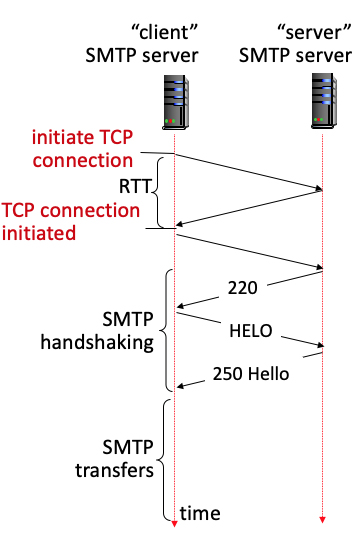
\includegraphics[width=.4\linewidth]{figs/2.3.1.jpg}
\end{center}

\item* 3
\item 0
\item 1
\item 2
\item 2.5
\end{multi}
        

\begin{multi}[points=1,shuffle,multiple]{2.3-2 Confronto tra HTTP e SMTP.}
\textbf{2.3-2 Confronto tra HTTP e SMTP.} 
Quali delle seguenti caratteristiche si applicano solo a HTTP (e \emph{non} si applicano a SMTP)?  
Nota: selezionare una o più delle caratteristiche di seguito.

\item Ha interazione in formato ASCII, con codici di stato.
\item Opera principalmente come un protocollo di push del client.
\item[fraction=33.33333] Opera principalmente come un protocollo di pull del client.
\item È in grado di utilizzare una connessione TCP persistente per trasferire più oggetti.
\item Utilizza CRLF.CRLF per indicare la fine del messaggio.
\item[fraction=33.33333] Utilizza una riga vuota (CRLF) per indicare la fine dell'intestazione della richiesta.
\item[fraction=33.33333] Utilizza la porta del server 80.
\item Utilizza la porta del server 25.
\end{multi}
            

\begin{multi}[points=1,shuffle,multiple]{2.3-3 Confronto tra HTTP e SMTP (2).}
\textbf{2.3-3 Confronto tra HTTP e SMTP (2).} 

Quali delle seguenti caratteristiche si applicano solo a SMTP (e \emph{non} si applicano a HTTP)?  
Nota: selezionare una o più delle caratteristiche di seguito.

\item Ha interazione in formato ASCII, con codici di stato.
\item[fraction=33.33333] Opera principalmente come un protocollo di push del client.
\item Opera principalmente come un protocollo di pull del client.
\item È in grado di utilizzare una connessione TCP persistente per trasferire più oggetti.
\item[fraction=33.33333] Utilizza CRLF.CRLF per indicare la fine del messaggio.
\item Utilizza una riga vuota (CRLF) per indicare la fine dell'intestazione della richiesta.
\item Utilizza la porta del server 80.
\item[fraction=33.33333] Utilizza la porta del server 25.
\end{multi}
    

\begin{multi}[points=1,shuffle,multiple]{2.3-4 Confronto tra HTTP e SMTP (3).}
\textbf{2.3-4 Confronto tra HTTP e SMTP (3).} 
Quali delle seguenti caratteristiche si applicano sia a HTTP che a SMTP? 
Nota: selezionare una o più delle caratteristiche di seguito.

\item[fraction=50] Ha interazione in formato ASCII, con codici di stato.
\item Opera principalmente come un protocollo di push del client.
\item Opera principalmente come un protocollo di pull del client.
\item[fraction=50] È in grado di utilizzare una connessione TCP persistente per trasferire più oggetti.
\item Utilizza CRLF.CRLF per indicare la fine del messaggio.
\item Utilizza una riga vuota (CRLF) per indicare la fine dell'intestazione della richiesta.
\end{multi}

\begin{matching}[points=1,shuffle]{2.3-5 Quale protocollo di posta elettronica?}
\textbf{2.3-5 Quale protocollo di posta elettronica?}  
Abbina la funzionalità di un protocollo al nome del protocollo di posta elettronica (se presente) che implementa quella funzionalità.
\item Fa push delle email da un client di posta a un server di posta. \answer SMTP
\item Preleva le email da un server di posta a un altro server di posta. \answer Né SMTP né IMAP fanno questo.
\item Preleva le email da un server di posta a un client di posta. \answer IMAP
\end{matching}
    
\begin{matching}[points=1,shuffle]{2.4-01 Funzioni del DNS.}
\textbf{2.4-01 Funzioni del DNS.} 
Abbinare la funzione di un server a un tipo di server DNS nell'organizzazione gerarchica dei server DNS.
\item Fornisce mappature autoritative dei nomi di host in indirizzi IP per gli host dell'organizzazione. \answer Server DNS autoritativo
\item Risponde alle query DNS dell'host locale, contattando altri server DNS per rispondere alla query. \answer Server DNS locale
\item Responsabile di un dominio (ad esempio, *.com, *.edu); sa come contattare i server DNS autoritativi. \answer Top-Level Domain Server (TLD)
\item Livello più alto dell'organizzazione DNS, sa come raggiungere i server responsabili di un determinato dominio (ad esempio, *.com, *.edu). \answer Root Server
\end{matching}
    
\begin{multi}[points=1,shuffle,multiple]{2.4-02 Perché il server DNS locale usa una cache?}
\textbf{2.4-02 Perché il server DNS locale usa una cache?} 
Qual è il valore della memorizzazione nella cache nel server DNS locale? Selezionare tutto ciò che si applica.

\item[fraction=50] La memorizzazione nella cache del DNS consente risposte più veloci, se la risposta alla query è presente nella cache.
\item[fraction=50] La memorizzazione nella cache del DNS comporta un carico inferiore altrove nel DNS, quando la risposta a una query è presente nella cache locale.
\item La memorizzazione nella cache del DNS fornisce accesso prioritario ai server radice, poiché la richiesta DNS proviene da una cache DNS locale.
\item La memorizzazione nella cache del DNS fornisce la capacità di fungere da server autoritativo per diverse organizzazioni.
\end{multi}

\begin{multi}[points=1,shuffle,multiple]{2.4-03 Cosa contiene il record di tipo A del DNS?}
\textbf{2.4-03 Cosa contiene il record di tipo A del DNS?} 
Quali informazioni contiene il record di tipo A nel database DNS? Selezionare tutto ciò che si applica.
\item* Un nome host e un indirizzo IP.
\item Un nome di dominio e il nome del server autoritativo per quel dominio.
\item Un nome di alias e un vero nome per un server.
\item Un nome e il nome del server SMTP associato a quel nome.
\end{multi}


\begin{multi}[points=1,shuffle,multiple]{2.4-04. Il server DNS locale.}
\textbf{2.4-04. Il server DNS locale.} 
Selezionare tutte le frasi seguenti che indicano una proprietà \emph{vera} di un server DNS \emph{locale}.
\item[fraction=50] Il record del server DNS locale per un host remoto è a volte diverso da quello del server autoritativo per quell'host.
\item Il server DNS locale viene contattato solo da un host locale se quell'host locale non è in grado di risolvere un nome tramite query iterative o ricorsive nella gerarchia del DNS.
\item Il server DNS locale detiene record di traduzione da nome host a indirizzo IP, ma non altri record DNS come i record MX.
\item[fraction=50] Il server DNS locale può diminuire il tempo di risoluzione da nome a indirizzo IP sperimentato da un host locale rispetto al caso in cui un DNS viene risolto tramite una query nella gerarchia del DNS.
\end{multi}


\begin{multi}[points=1,shuffle,multiple]{2.4-05. Server autoritativo.}
\textbf{2.4-05. Server autoritativo.} 
Qual è il ruolo di un server autoritativo nel DNS? (Selezionare tutto ciò che si applica.)
\item È un server locale (per l'host che effettua la query) che memorizza le coppie di traduzione da nome a indirizzo IP, in modo da poter rispondere in modo autorevole e rapidamente.
\item* Fornisce la risposta definitiva alla query riguardo a un nome nel dominio del server autoritativo.
\item Fornisce l'indirizzo IP del server DNS che può fornire la risposta definitiva alla query.
\item Fornisce un top-level domain (TLD) che possa essere interrogato per trovare l'indirizzo IP del server DNS che può fornire la risposta definitiva a questa query.
\end{multi}

\begin{multi}[points=1,shuffle]{2.4-06. Cache DNS.}
\textbf{2.4-06. Cache DNS.}
Abbiamo visto che una cache DNS locale risponderà immediatamente a un client quando la cache DNS locale ha la traduzione da nome a indirizzo. Ci sono milioni di queste cache DNS in tutto Internet. Per un dato nome Internet, la coppia di traduzione da nome a indirizzo memorizzata in queste cache sarà sempre la stessa (cioè, i contenuti delle cache sono sincronizzati)?

\item* \textbf{No.} Le cache non sono sempre sincronizzate. Una voce in una cache locale scadrà alla fine, e la cache andrà nuovamente alla gerarchia DNS per ottenere la coppia di traduzione da nome a indirizzo per questo nome. Quindi, se la mappatura da nome a indirizzo cambia nella gerarchia DNS, la nuova mappatura entrerà eventualmente (ma non immediatamente) nella cache. Pertanto, non tutte le cache avranno lo stesso valore per la coppia di traduzione da nome a indirizzo.
\item \textbf{No.} Le cache non sono sempre sincronizzate. Quando una mappatura da nome a indirizzo cambia nella gerarchia DNS, la gerarchia DNS farà \emph{push} della nuova mappatura in tutte le cache. Tuttavia, ci vogliono tempi diversi per la propagazione di questi aggiornamenti in tutte le cache. Di conseguenza, le cache non sono sempre perfettamente sincronizzate.
\item \textbf{Sì.} Le cache sono sempre sincronizzate. Quando una mappatura da nome a indirizzo cambia nella gerarchia DNS, la gerarchia DNS spingerà la nuova mappatura in tutte le cache, e le cache non installeranno la nuova mappatura fino a quando tutte le cache avranno apportato le modifiche.
\end{multi}

\begin{multi}[points=1,shuffle,multiple]{2.4-07. Caching DNS e HTTP.}
\textbf{2.4-07. Caching DNS e HTTP.}
Abbiamo imparato che la cache del browser web HTTP, la cache del server web locale HTTP e la cache DNS locale beneficiano gli utenti (ad esempio, perché riducono il ritardo di trasmissione). In quale delle seguenti forme di memorizzazione nella cache un utente beneficia non solo dalle proprie richieste recenti e dalle risposte memorizzate, \emph{ma anche dalle richieste recenti fatte da altri utenti}?
\item[fraction=50] Memorizzazione nella cache del server DNS locale
\item Memorizzazione nella cache del browser HTTP
\item[fraction=50] Memorizzazione nella cache del server web locale HTTP
\end{multi}


\begin{multi}[points=1,shuffle]{2.6-1 CDN.}
\textbf{2.6-1 CDN.}
Quale approccio adotta una CDN per trasmettere contenuti a centinaia di migliaia di utenti simultanei?
\item Servire video da un singolo ``mega-server'' centrale con connettività di rete ad altissima velocità e archiviazione ad alta velocità.
\item* Archiviare/servire copie multiple di video in siti distribuiti geograficamente.
\item Spingere proattivamente i video su un dispositivo client prima che vengano richiesti, utilizzando l'apprendimento automatico per prevedere i video richiesti.
\item Consentire ai dispositivi client di inviare il contenuto richiesto l'uno all'altro per alleggerire l'infrastruttura CDN.
\end{multi}


\begin{matching}[points=1,shuffle]{2.6-2 Definizioni di video in streaming.}
\textbf{2.6-2 Definizioni di video in streaming.}
Abbinare la definizione/funzione di un elemento o approccio in un sistema di video in streaming con il suo nome.
\item Un'unità di video, ognuna delle quali può essere codificata a velocità diverse, memorizzata in file diversi. \answer Chunk
\item Un file che contiene la posizione e la velocità di codifica dei file corrispondenti a segmenti video. \answer Manifest
\item Un approccio che consente a un client di adattare la velocità di codifica del video recuperato alle condizioni di congestione di rete. \answer DASH
\item Un approccio di CDN che memorizza contenuti nelle reti di accesso, vicino agli clienti. \answer ``Enter deep''
\item \answer Over The Top (OTT)
\item \answer Frame video
\end{matching}


\begin{multi}[points=1,shuffle]{2.6-3 Cosa è DASH?}
\textbf{2.6-3 Cosa è DASH?}
In DASH (Dynamic, Adaptive Streaming over HTTP), un server suddivide un file video in chunk che... (scegli il miglior completamento tra le seguenti opzioni)
\item* ...sono memorizzati, ognuno codificato a diverse velocità (qualità del video). Il client riproduce il video chunk per chunk, con ciascun chunk richiesto alla velocità di codifica che si adatta alla banda disponibile al momento.
\item ...sono scaricati a partire dal chunk più piccolo per massimizzare il numero di chunk ricevuti.
\item ...sono memorizzati, ognuno codificato a diverse velocità (qualità del video). Il client riceve più chunk video (codificati a diverse velocità) e riproduce i chunk che si adattano meglio alle dimensioni dello schermo.
\item ...vengono scaricati poco prima del loro tempo di riproduzione. La suddivisione è utilizzata principalmente perché uno spettatore potrebbe saltare avanti/indietro in un video.
\item ...permettono agli utenti premium di evitare di guardare chunk che contengono pubblicità.
\end{multi}

\begin{multi}[points=1,shuffle]{2.6-4 Manifest.}
\textbf{2.6-4 Manifest.}
Qual è lo scopo di un \emph{manifest} in un contesto di streaming multimediale?
\item Consente a un servizio video di registrare il video e il server da cui un client sta effettuando lo streaming di un video.
\item Permette a un client di riservare larghezza di banda lungo un percorso da un server a quel client, in modo che il client possa visualizzare uno streaming video senza problemi.
\item* Permette a un client di sapere dove può recuperare diversi segmenti video, codificati a diverse velocità.
\item Permette a un server video OTT (Over-the-top) di conoscere il video che il client desidera visualizzare.
\end{multi}

\begin{multi}[points=1,shuffle,multiple]{2.6-5. Streaming di Netflix.}
\textbf{2.6-5. Streaming di Netflix.}
Quali delle seguenti affermazioni (una o più) sono vere riguardo allo streaming di Netflix (seleziona tutte quelle vere) o ai servizi di streaming video in generale.
\item Una volta che un video inizia lo streaming da un server di Netflix, la qualità del video rimane costante per tutta la riproduzione del video.
\item Una volta che un video inizia lo streaming da un determinato server di Netflix, quel server sarà l'unico server assegnato a trasmettere quel video a quel client per l'intera sessione di visualizzazione di questo video.
\item* In Netflix, il client richiede chunk di video, e ciascun chunk può avere una diversa velocità di codifica (qualità del video) e può essere recuperato da un diverso server.
\end{multi}


\begin{multi}[points=1,shuffle,multiple]{2.7-1 Socket UDP.}
\textbf{2.7-1 Socket UDP.}
Quali delle seguenti caratteristiche seguenti sono associate a un socket UDP? Seleziona una o più opzioni che si applicano.
\item \emph{socket(AF\_INET, SOCK\_STREAM)} crea questo tipo di socket
\item[fraction=25] \emph{socket(AF\_INET, SOCK\_DGRAM)} crea questo tipo di socket
\item un server può eseguire un \emph{accept()} su questo tipo di socket
\item[fraction=25] fornisce il trasferimento non affidabile di gruppi di byte (datagramma) dal client al server
\item fornisce un trasferimento affidabile e in ordine di byte (un ``pipe'') dal client al server
\item[fraction=25] l'applicazione deve specificare esplicitamente l'indirizzo IP di destinazione e il numero di porta per ciascun gruppo di byte scritto in un socket
\item quando contattato, il server creerà un nuovo socket lato server per comunicare con quel client
\item[fraction=25] i dati provenienti da diversi client possono essere ricevuti sullo stesso socket
\end{multi}


\begin{multi}[points=1,shuffle,multiple]{2.7-2 Socket TCP.}
\textbf{2.7-2 Socket TCP.}
Quali delle seguenti caratteristiche seguenti sono associate a un socket TCP? Seleziona una o più opzioni che si applicano.
\item[fraction=25] \emph{socket(AF\_INET, SOCK\_STREAM)} crea questo tipo di socket
\item \emph{socket(AF\_INET, SOCK\_DGRAM)} crea questo tipo di socket
\item[fraction=25] un server può eseguire un \emph{accept()} su questo tipo di socket
\item fornisce il trasferimento non affidabile di gruppi di byte (datagramma) dal client al server
\item[fraction=25] fornisce un trasferimento affidabile e in ordine di byte (un ``pipe'') dal client al server
\item l'applicazione deve specificare esplicitamente l'indirizzo IP di destinazione e il numero di porta per ciascun gruppo di byte scritto in un socket
\item[fraction=25] quando contattato, il server creerà un nuovo socket lato server per comunicare con quel client
\item i dati provenienti da diversi client possono essere ricevuti sullo stesso socket
\end{multi}


\begin{multi}[points=1,shuffle]{2.7-3 Risposta del server (UDP).}
\textbf{2.7-3 Risposta del server (UDP).}
Come sa l'applicazione di rete in esecuzione su un server l'indirizzo IP del client e il numero di porta a cui rispondere in risposta a un datagramma ricevuto?
\item* Il codice dell'applicazione sul server determina l'indirizzo IP del client e il numero di porta dal segmento iniziale inviato dal client e deve specificare esplicitamente questi valori quando invia dati in un socket di ritorno a quel client.
\item Come risultato dell'esecuzione dell'istruzione \emph{accept()}, il server ha creato un nuovo socket legato a quel client specifico, quindi l'invio in questo nuovo socket (senza specificare esplicitamente l'indirizzo IP del client e il numero di porta) è sufficiente per garantire che i dati inviati saranno indirizzati al client corretto.
\item Il server interrogherà il DNS per conoscere l'indirizzo IP del client.
\item Il server conoscerà il numero di porta utilizzato dal client poiché tutti i servizi hanno un numero di porta ben noto.
\end{multi}

\begin{multi}[points=1,shuffle]{2.7-4 Quanti socket?}
\textbf{2.7-4 Quanti socket?}
Supponi che un server Web abbia \emph{cinque} connessioni in corso che utilizzano la porta di ricezione TCP 80 e supponi che non ci siano altre connessioni TCP (aperte o in fase di apertura o chiusura) in quel server. Quanti socket TCP sono in uso in questo server?
\item* 6
\item 1
\item 4
\item 5
\end{multi}

\begin{multi}[points=1,shuffle]{2.7-5 Procedura di \emph{connect()} del socket.}
\textbf{2.7-5 Procedura di \emph{connect()} del socket.}
Cosa succede quando viene chiamata/invocata la procedura \emph{connect()} di un socket?
\item* Questa procedura crea un nuovo socket sul client e connette quel socket al server specificato.
\item Questo fa sì che il client contatti un server TCP per stabilire una connessione tra quel client e il server. Se esiste già uno o più server su questa connessione, anche questo nuovo server verrà aggiunto a questa connessione.
\item Questo fa sì che il server contatti un client TCP per stabilire una connessione tra quel client e il server.
\end{multi}
                              
\end{quiz}
\end{document}
